\documentclass[11pt, a4paper]{article}

% Pacchetti base per lingua e codifica
\usepackage[utf8]{inputenc}
\usepackage[italian]{babel}

% Pacchetti per la matematica e la fisica
\usepackage{amsmath, amssymb, amsfonts}
\usepackage{cancel} % Utile per sbarrare i termini che si annullano

% Pacchetti per la grafica e l'impaginazione
\usepackage{graphicx}
\usepackage{geometry}
\geometry{top=2.5cm, bottom=2.5cm, left=2.5cm, right=2.5cm}
\usepackage{booktabs}
\usepackage{multirow}
\usepackage{sectsty}
\usepackage{float}
\usepackage{xcolor}
\allsectionsfont{\underline}
\setcounter{secnumdepth}{0}

\begin{document}
\tableofcontents

\newpage

\section{Rappresentazione Matriciale di Operatori e Funzioni d'Onda} %

Per comprendere a fondo la Meccanica Quantistica, è utilissimo tracciare un parallelo tra la normale geometria dei vettori e lo spazio delle funzioni d'onda. %

\begin{itemize}
    \item \textbf{Nello Spazio Vettoriale $\mathbb{C}^3$:} %
    Un vettore $\vec{f}$ è descritto dalle sue componenti in una certa base $\{\vec{u}_1, \vec{u}_2, \vec{u}_3\}$. 
\begin{figure}[H]
    \centering
    \begin{minipage}{0.3\textwidth}
        \centering
        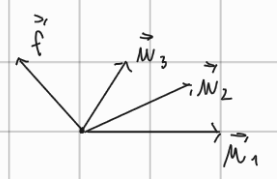
\includegraphics[width=\linewidth]{immagini/2026-05-22-14-31-05.png}
    \end{minipage}\hfill
    \begin{minipage}{0.65\textwidth}
            \begin{equation*}
                \vec{f} = \begin{pmatrix} f_x \\ f_y \\ f_z \end{pmatrix} \equiv |\vec{f}\rangle \quad \Leftrightarrow \quad \langle\vec{f}| \equiv \vec{f}^{*T} = \begin{pmatrix} f_x^* & f_y^* & f_z^* \end{pmatrix} %
            \end{equation*}
    \end{minipage}
\end{figure}
    Il prodotto scalare è $\langle\vec{g}|\vec{f}\rangle$, e i vettori si trasformano tramite \textbf{Matrici $\hat{M}$}. %

    \item \textbf{Nello Spazio Funzionale $\mathcal{L}^2$:} %
    Una funzione $f(x)$ può essere vista come un vettore con infinite componenti continue. %
    \begin{figure}[H]
        \centering
        \begin{minipage}{0.3\textwidth}
            \centering
            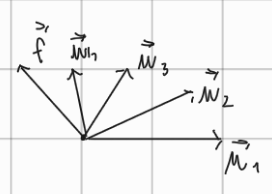
\includegraphics[width=\linewidth]{immagini/2026-05-22-14-31-50.png}
        \end{minipage}\hfill
        \begin{minipage}{0.65\textwidth}
            \begin{equation*}
                |f\rangle \quad \Leftrightarrow \quad \langle f| = f^* \quad \Rightarrow \quad \langle f|g\rangle = \int f^* g \, dx %
            \end{equation*}
        \end{minipage}
    \end{figure}
    Scegliendo una base di funzioni $\{u_n\}$, possiamo espandere lo stato come $|f\rangle = \sum c_n |u_n\rangle$. Qui le funzioni si trasformano tramite \textbf{Operatori $\hat{O}$} (es. derivate). %
\end{itemize}

\noindent
L'incredibile intuizione di Dirac fu quella di unire queste due visioni in un unico contenitore: lo \textbf{Spazio Astratto dei KET $\mathcal{H}$} (Spazio di Hilbert). %

\subsection{Proprietà dello Spazio dei Ket} %

Lo spazio $\mathcal{H}$ è uno spazio vettoriale complesso i cui elementi sono indicati con $|\Psi\rangle$. Gode delle seguenti proprietà: %
\begin{enumerate}
    \item \textbf{Linearità:} $|\chi\rangle = \alpha|\Psi\rangle + \beta|\varphi\rangle$ (con $\alpha, \beta \in \mathbb{C}$). %
    \item \textbf{Dualità Bra-Ket:} Ad ogni Ket $|\cdot\rangle$ corrisponde biunivocamente un Bra $\langle\cdot|$, che ne rappresenta il trasposto complesso coniugato ($|\cdot\rangle^{*T} \equiv |\cdot\rangle^\dagger$). %
    \item \textbf{Prodotto Interno:} Genera uno scalare complesso ed è hermitiano: $\langle\varphi|\Psi\rangle = \langle\Psi|\varphi\rangle^*$. %
    \item \textbf{Completezza:} Lo spazio è completo rispetto alla norma indotta dal prodotto scalare: $||\Psi|| = \sqrt{\langle\Psi|\Psi\rangle}$. %
    \item \textbf{Esistenza di una Base:} Esiste un set di Ket base $\{|u_n\rangle\}$ ortonormali ($\langle u_n|u_m\rangle = \delta_{nm}$) tale che ogni stato possa essere scritto come $|\Psi\rangle = \sum c_n |u_n\rangle$. %
\end{enumerate}
\textit{Finché non scelgo una base precisa, il Ket rimane un oggetto astratto.} %
\subsection{Scelta della Base e Vettori Colonna} %

Se scegliamo una base specifica $\{|u_i\rangle\}$, possiamo proiettare il nostro stato astratto su di essa. Moltiplicando a sinistra per un bra della base $\langle u_k|$, per l'ortonormalità sopravvive solo il coefficiente $k$-esimo: %
\begin{equation}
    |f\rangle = \sum_i c_i |u_i\rangle \quad \Rightarrow \quad \boxed{ c_i = \langle u_i|f\rangle } %
\end{equation}

\textbf{Esempi:} %
\begin{itemize}
    \item Vettore 3D ordinario: $|\vec{v}\rangle = 2|\vec{u}_1\rangle + 3|\vec{u}_2\rangle + 4|\vec{u}_3\rangle \Rightarrow |\vec{v}\rangle = \begin{pmatrix} 2 \\ 3 \\ 4 \end{pmatrix}$ %
    \item Stato quantistico (Armoniche Sferiche per $l=1$): %
    \begin{equation*}
        |\Psi\rangle = \sqrt{\frac{3}{5}} |Y_1^1\rangle + \sqrt{\frac{1}{5}} |Y_1^0\rangle + \sqrt{\frac{1}{5}} |Y_1^{-1}\rangle \quad \Rightarrow \quad |\Psi\rangle = \begin{pmatrix} \sqrt{3/5} \\ \sqrt{1/5} \\ \sqrt{1/5} \end{pmatrix} %
    \end{equation*}
\end{itemize}

\noindent
\textbf{Conclusione fondamentale:} Fissata una base, il vettore colonna dei coefficienti $\begin{pmatrix} c_1, c_2, \dots, c_n \end{pmatrix}^T$ determina \textbf{univocamente} lo stato quantistico. La dimensione della colonna è data dal numero $n$ di componenti della base. %

\subsection{Gli Operatori diventano Matrici} %

Vediamo come agisce un operatore $\hat{O}$ su uno stato $|\Psi\rangle$ per trasformarlo in un nuovo stato $|\varphi\rangle$: %
\begin{equation*}
    |\varphi\rangle = \hat{O}|\Psi\rangle %
\end{equation*}

\noindent
Sostituiamo l'espressione di $|\Psi\rangle$ espansa nella base: %
\begin{equation*}
    |\varphi\rangle = \hat{O} \left( \sum_j c_j |u_j\rangle \right) = \sum_j c_j \hat{O} |u_j\rangle %
\end{equation*}

\noindent
Vogliamo trovare i coefficienti del \textit{nuovo} vettore $|\varphi\rangle$ in questa base. Chiamiamo $b_i$ la proiezione di $|\varphi\rangle$ sull'$i$-esimo vettore di base. Moltiplichiamo tutto a sinistra per il bra $\langle u_i|$: %
\begin{equation}
    b_i = \langle u_i|\varphi\rangle = \langle u_i| \left( \sum_j c_j \hat{O} |u_j\rangle \right) = \sum_j c_j \underbrace{ \langle u_i|\hat{O}|u_j\rangle }_{O_{ij}} %
\end{equation}

\noindent
Il termine incastrato nel mezzo, $\langle u_i|\hat{O}|u_j\rangle$, è un numero (uno scalare complesso) ed è definito come \textbf{ELEMENTO DI MATRICE} $O_{ij}$ dell'operatore $\hat{O}$. %

\noindent
L'equazione $b_i = \sum_j O_{ij} c_j$ è l'esatta definizione del prodotto riga per colonna dell'algebra lineare! %
Possiamo riscrivere l'intera operazione vettoriale $|\varphi\rangle = \hat{O}|\Psi\rangle$ in forma esplicita matriciale: %

\begin{equation}
    \begin{pmatrix} b_1 \\ b_2 \\ \vdots \\ b_i \\ \vdots \end{pmatrix} = \begin{pmatrix} (\hat{O}\Psi)_1 \\ (\hat{O}\Psi)_2 \\ \vdots \\ (\hat{O}\Psi)_i \\ \vdots \end{pmatrix} = \begin{bmatrix} O_{11} & O_{12} & \dots & O_{1j} & \dots \\ O_{21} & O_{22} & \dots & O_{2j} & \dots \\ \vdots & \vdots & \ddots & \vdots & \\ O_{i1} & O_{i2} & \dots & O_{ij} & \dots \\ \vdots & \vdots & & \vdots & \ddots \end{bmatrix} \begin{pmatrix} c_1 \\ c_2 \\ \vdots \\ c_j \\ \vdots \end{pmatrix} %
\end{equation}

\begin{quote}
    \textbf{Il trionfo della Meccanica delle Matrici:} %
    Abbiamo trasformato un \textbf{Operatore Differenziale} (che per agire richiede il calcolo di integrali e derivate su funzioni d'onda continue) in una banale \textbf{Matrice} $N \times N$ che agisce su un \textbf{Vettore colonna} di coefficienti! %
\end{quote}
Se la base scelta ha dimensione $N$, la matrice dell'operatore sarà una matrice quadrata $N \times N$. Questo è il motivo per cui, ad esempio nello Spin dell'elettrone ($N=2$), gli operatori $\hat{S}_x, \hat{S}_y, \hat{S}_z$ sono rappresentati dalle Matrici di Pauli $2 \times 2$. %


\subsection{Risoluzione dell'Identità e Prodotto di Operatori} %

Riprendiamo lo sviluppo di uno stato nella base: %
\begin{equation*}
    |\Psi\rangle = \sum_i c_i |u_i\rangle = \sum_i |u_i\rangle \langle u_i|\Psi\rangle = \left( \sum_i |u_i\rangle \langle u_i| \right) |\Psi\rangle %
\end{equation*}
L'operatore tra parentesi lascia inalterato lo stato $|\Psi\rangle$, quindi rappresenta l'\textbf{Operatore Identità} $\hat{I}$: %
\begin{equation}
    \boxed{ \sum_i |u_i\rangle \langle u_i| = \hat{I} } \quad \text{(Relazione di Completezza o Risoluzione dell'Identità)} %
\end{equation}

\noindent
Questa relazione è un "trucco" potentissimo. Vediamo cosa succede se applichiamo due operatori in sequenza ($\hat{O}\hat{P}$) e calcoliamo il loro elemento di matrice $\langle u_k | \hat{O}\hat{P} | u_j \rangle$. %
Possiamo inserire l'identità $\hat{I} = \sum_i |u_i\rangle \langle u_i|$ proprio in mezzo ai due operatori: %
\begin{equation*}
    \langle u_k | \hat{O} \hat{I} \hat{P} | u_j \rangle = \sum_i \underbrace{ \langle u_k | \hat{O} | u_i \rangle }_{O_{ki}} \underbrace{ \langle u_i | \hat{P} | u_j \rangle }_{P_{ij}} = \sum_i O_{ki} P_{ij} %
\end{equation*}

\noindent
Questo dimostra formalmente che l'azione successiva di due operatori differenziali equivale esattamente al \textbf{prodotto riga per colonna tra le due matrici corrispondenti}: %
\begin{equation}
    (\hat{O}\hat{P})_{kj} = \sum_i O_{ki} P_{ij} \quad \Rightarrow \quad \text{Il prodotto tra due operatori diventa un prodotto tra matrici!} %
\end{equation}

\noindent
Analogamente, per l'operatore aggiunto (Ermitiano Coniugato $\hat{O}^\dagger$): %
\begin{equation}
    (\hat{O}^\dagger)_{ij} = \langle u_i | \hat{O}^\dagger | u_j \rangle = \langle \hat{O} u_i | u_j \rangle = \langle u_j | \hat{O} | u_i \rangle^* = O_{ji}^* %
\end{equation}
La matrice dell'operatore aggiunto è la matrice trasposta complessa coniugata. %

\begin{itemize}
    \item Se scegliamo come base proprio il \textbf{set degli autostati dell'operatore $\hat{O}$}, allora la sua matrice sarà perfettamente diagonale: %
\begin{equation*}
    \langle u_i | \hat{O} | u_j \rangle = \langle u_i | O_j | u_j \rangle = O_j \langle u_i | u_j \rangle = O_j \delta_{ij} %
\end{equation*}
    \item Se $\vec{O}$ ha uno spettro di autostati discreto allora sarà rappresentato da una matrice $NxN$, se inveca ha spettro continuo non può essere rappresentato da una matrice essendo un inf. non numerabile.
\end{itemize}


\noindent
\textbf{Esempio di Rappresentazione Matriciale:} %
Costruiamo le matrici del momento angolare orbitale $\vec{L}$ per lo stato $l=1$. %
La base degli autostati di $\hat{L}^2$ e $\hat{L}_z$ è formata da tre vettori (Armoniche Sferiche $Y^m_{l}$): $|1, 1\rangle, |1, 0\rangle, |1, -1\rangle$. %
Un ket generico sarà: %
\begin{equation*}
    |\Psi\rangle = \alpha |1, 1\rangle + \beta |1, 0\rangle + \gamma |1, -1\rangle \quad \Rightarrow \quad |\Psi\rangle = \begin{pmatrix} \alpha \\ \beta \\ \gamma \end{pmatrix} %
\end{equation*}

\noindent
L'operatore $\hat{L}_z$ su questa base è \textbf{diagonale}, poiché l'equazione agli autovalori è $\hat{L}_z |l, m\rangle = \hbar m |l, m\rangle$. Gli elementi di matrice sono: %
\begin{equation*}
    \langle 1, m' | \hat{L}_z | 1, m \rangle = \hbar m \delta_{m',m} %
\end{equation*}
Costruiamo esplicitamente la matrice $3 \times 3$: %
\begin{equation}
    L_z = \begin{pmatrix} \langle 1,1|\hat{L}_z|1,1\rangle & \langle 1,1|\hat{L}_z|1,0\rangle & \langle 1,1|\hat{L}_z|1,-1\rangle \\ \langle 1,0|\hat{L}_z|1,1\rangle & \langle 1,0|\hat{L}_z|1,0\rangle & \langle 1,0|\hat{L}_z|1,-1\rangle \\ \langle 1,-1|\hat{L}_z|1,1\rangle & \langle 1,-1|\hat{L}_z|1,0\rangle & \langle 1,-1|\hat{L}_z|1,-1\rangle \end{pmatrix} = \begin{pmatrix} \hbar & 0 & 0 \\ 0 & 0 & 0 \\ 0 & 0 & -\hbar \end{pmatrix} = \hbar \begin{pmatrix} 1 & 0 & 0 \\ 0 & 0 & 0 \\ 0 & 0 & -1 \end{pmatrix} %
\end{equation}

\noindent
Per trovare le matrici di $\hat{L}_x$ e $\hat{L}_y$, sfruttiamo gli operatori di salita e discesa ($\hat{L}_+$ e $\hat{L}_-$), per i quali valgono le equazioni: %
\begin{align*}
    \hat{L}_+ |l, m\rangle &= \hbar \sqrt{l(l+1) - m(m+1)} |l, m+1\rangle \\ %
    \hat{L}_- |l, m\rangle &= \hbar \sqrt{l(l+1) - m(m-1)} |l, m-1\rangle %
\end{align*}

\noindent
Calcolando gli elementi di matrice per $l=1$, otteniamo che $\hat{L}_+$ ha elementi non nulli solo per $m' = m+1$ (sopradiagonale), e $\hat{L}_-$ per $m' = m-1$ (sottodiagonale): %
\begin{equation}
    L_+ = \hbar \begin{pmatrix} 0 & \sqrt{2} & 0 \\ 0 & 0 & \sqrt{2} \\ 0 & 0 & 0 \end{pmatrix} \quad , \quad L_- = \hbar \begin{pmatrix} 0 & 0 & 0 \\ \sqrt{2} & 0 & 0 \\ 0 & \sqrt{2} & 0 \end{pmatrix} %
\end{equation}

\noindent
Sapendo che $\hat{L}_x = \frac{1}{2}(\hat{L}_+ + \hat{L}_-)$ e $\hat{L}_y = \frac{1}{2i}(\hat{L}_+ - \hat{L}_-)$, deriviamo le matrici finali non diagonali: %
\begin{equation}
    \boxed{ \hat{L}_x = \frac{\hbar}{\sqrt{2}} \begin{pmatrix} 0 & 1 & 0 \\ 1 & 0 & 1 \\ 0 & 1 & 0 \end{pmatrix} } \qquad , \qquad \boxed{ \hat{L}_y = \frac{\hbar}{i\sqrt{2}} \begin{pmatrix} 0 & 1 & 0 \\ -1 & 0 & 1 \\ 0 & -1 & 0 \end{pmatrix} = \frac{\hbar}{\sqrt{2}} \begin{pmatrix} 0 & -i & 0 \\ i & 0 & -i \\ 0 & i & 0 \end{pmatrix} } %
\end{equation}

\noindent
\textit{Nota:} Se fossimo passati a $l=2$, le matrici sarebbero state di dimensione $5 \times 5$ (poiché $m_l = -2, -1, 0, 1, 2$). Se andiamo a $s=1/2$, la dimensione è $2 \times 2$, e ricadiamo esattamente nelle Matrici di Pauli per lo Spin! %

\subsection{Operatori a Spettro Continuo: La Funzione d'Onda} %

Abbiamo visto che per operatori con spettro \textbf{discreto} (es. $\hat{L}_z$), lo stato è un vettore colonna a $N$ componenti, e l'operatore una matrice $N \times N$. %

\noindent
Ma cosa succede per l'operatore posizione $\hat{x}$, che ha uno spettro \textbf{continuo}? %
L'indice di base $i$ discreto diventa una variabile continua $x$. La sommatoria diventa un integrale. Lo stato astratto $|\Psi\rangle$ si espande in una base di infiniti autoket della posizione $|x\rangle$: %
\begin{equation*}
    |\Psi\rangle = \int c(x) |x\rangle \, dx %
\end{equation*}

\noindent
L'ortonormalità discreta ($\delta_{ij}$) diventa l'ortonormalità continua della Delta di Dirac ($\delta(x-x')$): %
\begin{equation*}
    \langle x | x' \rangle = \delta(x-x') %
\end{equation*}

\noindent
Per trovare il "coefficiente" $c(x)$, proiettiamo il ket $|\Psi\rangle$ sulla base $\langle x|$: %
\begin{equation*}
    \langle x | \Psi \rangle = \int c(x') \langle x | x' \rangle \, dx' = \int c(x') \delta(x-x') \, dx' = c(x) %
\end{equation*}

\noindent
Poiché il modulo quadro di questo coefficiente $|c(x)|^2$ rappresenta la probabilità di misura (esattamente come $|c_i|^2$ nel caso discreto), \textbf{questo coefficiente continuo coincide con la Funzione d'Onda di Schrödinger}: %
\begin{equation}
    \boxed{ \Psi(x) = \langle x | \Psi \rangle } %
\end{equation}

\noindent
La funzione d'onda $\Psi(x)$ è semplicemente la rappresentazione del vettore di stato $|\Psi\rangle$ proiettato nella base delle coordinate spaziali! %
\begin{equation*}
    |\Psi\rangle = \begin{pmatrix} \Psi(x_1) \\ \Psi(x_2) \\ \vdots \\ \Psi(x_N) \end{pmatrix} \quad \text{un vettore colonna di altezza NON numerabile!} %
\end{equation*}

\section{Teoria delle Perturbazioni Non Dipendenti dal Tempo} %
\subsection{Stati Non Degeneri} %

Partiamo da un sistema fisico la cui Hamiltoniana Imperturbata $\hat{H}^{(0)}$ ci permette di risolvere l'equazione di Schrödinger in modo analitico e \textbf{esatto}: %
\begin{equation*}
    \hat{H}^{(0)} u_n^{(0)} = E_n^{(0)} u_n^{(0)} %
\end{equation*}
Conosciamo perfettamente i suoi autostati $u_n^{(0)}$ e i suoi autovalori $E_n^{(0)}$. %
Essendo base ortonormale: $\langle u_n^{(0)} | u_m^{(0)} \rangle = \int u_n^{(0)*} u_m^{(0)} d\tau = \delta_{nm}$ e $\langle u_n^{(0)} | \hat{H}^{(0)} | u_m^{(0)} \rangle = E_n^{(0)} \delta_{nm}$. \\

\noindent
\textbf{Esempio: Buca di Potenziale Infinita (0, a)} %
\begin{equation*}
    u_n^{(0)}(x) = \sqrt{\frac{2}{a}} \sin\left(\frac{n\pi x}{a}\right) \quad , \quad E_n^{(0)} = \frac{\pi^2 \hbar^2 n^2}{2m a^2} \qquad \text{con } n = 1, 2, 3 \dots %
\end{equation*}

\noindent
Aggiungiamo ora una piccola variazione al potenziale (una \textbf{Perturbazione} $\hat{H}'$). %
Nel nostro esempio, alziamo il fondo della buca di una quantità $V_0$ solo nella prima metà della buca: %
\begin{figure}[H]
    \centering
    \begin{minipage}{0.3\textwidth}
        \centering
        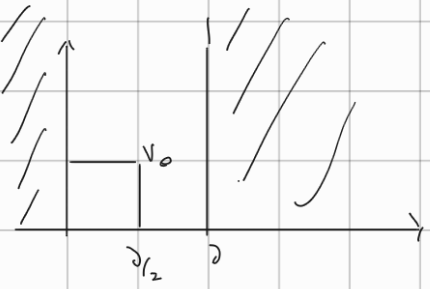
\includegraphics[width=\linewidth]{immagini/2026-05-22-15-02-02.png}
    \end{minipage}\hfill
    \begin{minipage}{0.65\textwidth}
        \begin{equation*}
            \hat{H}' = \hat{V}(x) = \begin{cases} V_0 & 0 \le x \le a/2 \\ 0 & \text{altrove} \end{cases} %
        \end{equation*}
    \end{minipage}
\end{figure}

\noindent
Il sistema perturbato totale avrà un'Hamiltoniana $\hat{H} = \hat{H}^{(0)} + \lambda \hat{H}'$, dove $\lambda$ è un parametro matematico fittizio molto piccolo ($\lambda \ll 1$), che garantisce che la perturbazione sia piccola rispetto al sistema ($\lambda\hat{H}' \ll \hat{H}^{(0)}$). %

\noindent
Vogliamo trovare le nuove soluzioni per l'equazione $\hat{H} u_n = E_n u_n$. Poiché non possiamo calcolarle in modo esatto, espandiamo sia la funzione d'onda che l'energia in \textbf{Serie di Potenze del parametro $\mathbf{\lambda}$}: %
\begin{align}
    u_n &= u_n^{(0)} + \lambda u_n^{(1)} + \lambda^2 u_n^{(2)} + \dots \\ %
    E_n &= E_n^{(0)} + \lambda E_n^{(1)} + \lambda^2 E_n^{(2)} + \dots %
\end{align}
\textit{L'esponente $(k)$ tra parentesi indica l'ordine della correzione.} %

\subsection{Uguaglianza dei Coefficienti} %

Sostituiamo gli sviluppi in serie nell'equazione di Schrödinger perturbata $\hat{H} u_n = E_n u_n$: %
\begin{equation*}
    \left[ \hat{H}^{(0)} + \lambda \hat{H}' \right] \left[ u_n^{(0)} + \lambda u_n^{(1)} + \lambda^2 u_n^{(2)} \dots \right] = \left[ E_n^{(0)} + \lambda E_n^{(1)} + \lambda^2 E_n^{(2)} \dots \right] \left[ u_n^{(0)} + \lambda u_n^{(1)} + \lambda^2 u_n^{(2)} \dots \right] %
\end{equation*}

Eseguiamo i prodotti, fermandoci per semplicità ai termini di secondo grado in $\lambda$: %
\begin{align*}
    & \hat{H}^{(0)}u_n^{(0)} + \lambda\hat{H}^{(0)}u_n^{(1)} + \lambda^2\hat{H}^{(0)}u_n^{(2)} + \lambda\hat{H}'u_n^{(0)} + \lambda^2\hat{H}'u_n^{(1)} + \dots = \\ %
    &= E_n^{(0)}u_n^{(0)} + \lambda E_n^{(0)}u_n^{(1)} + \lambda^2 E_n^{(0)}u_n^{(2)} + \lambda E_n^{(1)}u_n^{(0)} + \lambda^2 E_n^{(1)}u_n^{(1)} + \lambda^2 E_n^{(2)}u_n^{(0)} + \dots %
\end{align*}

Ora raccogliamo a fattore comune i termini con la stessa potenza di $\lambda$ da ambo i lati: %
\begin{align*}
    & \underbrace{ \hat{H}^{(0)}u_n^{(0)} }_{\lambda^0} + \lambda \underbrace{ \left[ \hat{H}^{(0)}u_n^{(1)} + \hat{H}'u_n^{(0)} \right] }_{\text{1° pot. } \lambda} + \lambda^2 \underbrace{ \left[ \hat{H}^{(0)}u_n^{(2)} + \hat{H}'u_n^{(1)} \right] }_{\text{2° pot. } \lambda} + \dots = \\ %
    &= \underbrace{ E_n^{(0)}u_n^{(0)} }_{\lambda^0} + \lambda \underbrace{ \left[ E_n^{(0)}u_n^{(1)} + E_n^{(1)}u_n^{(0)} \right] }_{\text{1° pot. } \lambda} + \lambda^2 \underbrace{ \left[ E_n^{(0)}u_n^{(2)} + E_n^{(1)}u_n^{(1)} + E_n^{(2)}u_n^{(0)} \right] }_{\text{2° pot. } \lambda} + \dots %
\end{align*}

\noindent
Affinché questa uguaglianza valga per qualsiasi valore di $\lambda$, i coefficienti delle corrispondenti potenze di $\lambda$ devono essere identici. Otteniamo così un sistema di equazioni differenziali a cascata: %
\begin{align}
    \text{Ordine } \lambda^0 &: \quad \hat{H}^{(0)} u_n^{(0)} = E_n^{(0)} u_n^{(0)} \quad \text{(Equazione Imperturbata Nota)} \\ %
    \text{Ordine } \lambda^1 &: \quad \hat{H}^{(0)} u_n^{(1)} + \hat{H}' u_n^{(0)} = E_n^{(0)} u_n^{(1)} + E_n^{(1)} u_n^{(0)} \\ %
    \text{Ordine } \lambda^2 &: \quad \hat{H}^{(0)} u_n^{(2)} + \hat{H}' u_n^{(1)} = E_n^{(0)} u_n^{(2)} + E_n^{(1)} u_n^{(1)} + E_n^{(2)} u_n^{(0)} %
\end{align}

\subsection{Correzione dell'Energia al Primo Ordine} %

Prendiamo l'equazione del primo ordine ($\lambda^1$). Per isolare la correzione dell'energia $E_n^{(1)}$, moltiplichiamo tutta l'equazione a sinistra per il bra complesso coniugato imperturbato $u_n^{(0)*}$ e integriamo su tutto lo spazio (proiezione): %
\begin{equation*}
    \langle u_n^{(0)} | \hat{H}^{(0)} | u_n^{(1)} \rangle + \langle u_n^{(0)} | \hat{H}' | u_n^{(0)} \rangle = E_n^{(0)} \langle u_n^{(0)} | u_n^{(1)} \rangle + E_n^{(1)} \underbrace{ \langle u_n^{(0)} | u_n^{(0)} \rangle }_{=1} %
\end{equation*}

\noindent
Poiché l'operatore $\hat{H}^{(0)}$ è hermitiano, può agire indifferentemente a sinistra sul bra: $\langle u_n^{(0)} | \hat{H}^{(0)} = \langle \hat{H}^{(0)} u_n^{(0)} | = E_n^{(0)} \langle u_n^{(0)} |$. Sostituiamo nel primo termine: %
\begin{equation*}
    \cancel{E_n^{(0)} \langle u_n^{(0)} | u_n^{(1)} \rangle} + \langle u_n^{(0)} | \hat{H}' | u_n^{(0)} \rangle = \cancel{E_n^{(0)} \langle u_n^{(0)} | u_n^{(1)} \rangle} + E_n^{(1)} %
\end{equation*}

\noindent
I due termini misti si elidono magicamente! Rimane la formula risolutiva fondamentale per la Correzione dell'Energia al 1° Ordine: %
\begin{equation}
    \boxed{ E_n^{(1)} = \langle u_n^{(0)} | \hat{H}' | u_n^{(0)} \rangle = \int_{\mathbb{R}} u_n^{(0)*} \hat{H}' u_n^{(0)} \, dx } %
\end{equation}
\textit{Il salto energetico è pari al valore di aspettazione (elemento di matrice diagonale) della perturbazione calcolato sugli stati imperturbati vecchi.} \\

\noindent
\textbf{Applicazione all'Esempio della Buca:} %
Calcoliamo $E_n^{(1)}$ per il gradino $V_0$ presente solo tra $0$ e $a/2$: %
\begin{equation*}
    E_n^{(1)} = \int_0^{a/2} u_n^{(0)*} (V_0) u_n^{(0)} \, dx = V_0 \int_0^{a/2} |u_n^{(0)}|^2 \, dx = V_0 \int_0^{a/2} \frac{2}{a} \sin^2\left(\frac{n\pi x}{a}\right) \, dx %
\end{equation*}
Essendo la funzione d'onda seno al quadrato perfettamente simmetrica rispetto al centro della buca, l'integrale su metà dominio restituisce esattamente la metà della probabilità totale (che è $1$): %
\begin{equation*}
    E_n^{(1)} = V_0 \left( \frac{1}{2} \right) = \frac{V_0}{2} %
\end{equation*}

\noindent
Ponendo alla fine $\lambda=1$, l'\textbf{Autovalore Imperturbato Corretto (Approssimato)} per l'energia diventa: %
\begin{equation}
    E_n \simeq E_n^{(0)} + \lambda E_n^{(1)} \quad \Rightarrow \quad \boxed{ E_n \simeq \frac{\hbar^2 \pi^2 n^2}{2m a^2} + \frac{V_0}{2} } %
\end{equation}

\begin{quote}
    \textbf{Condizioni di Esistenza (Perché l'integrale non si annulli):} %
    1. Il dominio della perturbazione $\hat{H}'$ si deve sovrapporre spazialmente ad $u_n^{(0)}$. % \\
    2. Questione di Parità: se $\hat{H}'$ e $u_n^{(0)}$ hanno parità differente in un dominio simmetrico, l'integrale del loro prodotto si annulla identicamente ($\int dx = 0$). %
\end{quote}

\subsection{Correzione della Funzione d'Onda al Primo Ordine} %

Riprendiamo l'equazione di Schrödinger perturbata al primo ordine in $\lambda$: %
\begin{equation*}
    \hat{H}^{(0)} u_n^{(1)} + \hat{H}' u_n^{(0)} = E_n^{(0)} u_n^{(1)} + E_n^{(1)} u_n^{(0)} %
\end{equation*}

\noindent
Riorganizziamo i termini per raggruppare l'incognita $u_n^{(1)}$ a sinistra e i termini noti a destra: %
\begin{equation}
    \underbrace{ \left[ \hat{H}^{(0)} - E_n^{(0)} \right] }_{\text{Operatore}} u_n^{(1)} = \underbrace{ -\left[ \hat{H}' - E_n^{(1)} \right] u_n^{(0)} }_{\text{Termine Noto}} %
\end{equation}

\noindent
Sappiamo che le autofunzioni imperturbate $u_m^{(0)}$ formano una base completa. Possiamo quindi esprimere la correzione incognita $u_n^{(1)}$ come combinazione lineare di questa base: %
\begin{equation*}
    u_n^{(1)} = \sum_m c_m u_m^{(0)} %
\end{equation*}

\noindent
Tuttavia, notiamo che la funzione $u_n^{(0)}$ appartiene al \textit{Kernel} (spazio nullo) dell'operatore a sinistra, poiché $[\hat{H}^{(0)} - E_n^{(0)}] u_n^{(0)} = 0$. %
Visto che $u_n^{(0)}$ si annulla applicando l'operatore, il suo coefficiente $c_n$ è arbitrario (rappresenta solo una ridefinizione della normalizzazione). Possiamo quindi escluderlo dalla sommatoria ponendo $c_n = 0$: %
\begin{equation}
    \Rightarrow \quad u_n^{(1)} = \sum_{m \neq n} c_m u_m^{(0)} %
\end{equation}

\noindent
Sostituiamo questo sviluppo nell'equazione riorganizzata: %
\begin{equation*}
    \left[ \hat{H}^{(0)} - E_n^{(0)} \right] \sum_{m \neq n} c_m u_m^{(0)} = -\left[ \hat{H}' - E_n^{(1)} \right] u_n^{(0)} %
\end{equation*}

\noindent
Poiché $\hat{H}^{(0)} u_m^{(0)} = E_m^{(0)} u_m^{(0)}$, l'operatore agisce sulla sommatoria trasformandosi nei rispettivi autovalori: %
\begin{equation*}
    \Rightarrow \quad \sum_{m \neq n} c_m \left( E_m^{(0)} - E_n^{(0)} \right) u_m^{(0)} = - \hat{H}' u_n^{(0)} + E_n^{(1)} u_n^{(0)} %
\end{equation*}

\noindent
Per trovare i coefficienti $c_m$, moltiplichiamo tutta l'equazione a sinistra per un generico bra imperturbato $\langle u_l^{(0)} |$ e integriamo su tutto lo spazio: %
\begin{equation*}
    \sum_{m \neq n} c_m \left( E_m^{(0)} - E_n^{(0)} \right) \underbrace{ \langle u_l^{(0)} | u_m^{(0)} \rangle }_{\delta_{lm}} = - \langle u_l^{(0)} | \hat{H}' | u_n^{(0)} \rangle + E_n^{(1)} \underbrace{ \langle u_l^{(0)} | u_n^{(0)} \rangle }_{\delta_{ln}} %
\end{equation*}

Analizziamo i due casi possibili per $l$: %
\begin{itemize}
    \item \textbf{Se $\mathbf{l = n}$:} La parte sinistra si annulla (poiché la somma esclude $m=n$). A destra sopravvive $\delta_{nn}=1$, ottenendo $0 = -\langle u_n^{(0)}|\hat{H}'|u_n^{(0)}\rangle + E_n^{(1)}$, che ci ridà la formula per l'energia al 1° ordine! %
    \item \textbf{Se $\mathbf{l \neq n}$:} Il secondo termine a destra si annulla ($\delta_{ln}=0$). A sinistra, la somma collassa all'unico termine per cui $m=l$, restituendo: %
    \begin{equation*}
        c_l \left( E_l^{(0)} - E_n^{(0)} \right) = - \langle u_l^{(0)} | \hat{H}' | u_n^{(0)} \rangle \quad \Rightarrow \quad c_l = \frac{ \langle u_l^{(0)} | \hat{H}' | u_n^{(0)} \rangle }{ E_n^{(0)} - E_l^{(0)} } %
    \end{equation*}
\end{itemize}

\noindent
Sostituendo i coefficienti trovati nella sommatoria iniziale, otteniamo la \textbf{Formula per la Correzione della Funzione d'Onda al 1° Ordine}: %
\begin{equation}
    \boxed{ u_n^{(1)} = \sum_{m \neq n} \frac{\langle u_m^{(0)} | \hat{H}' | u_n^{(0)} \rangle}{E_n^{(0)} - E_m^{(0)}} u_m^{(0)} } %
\end{equation}
\textit{Nota: $n$ è lo stato che sto correggendo, $m$ sono tutti gli altri autostati della base con cui lo correggo.} %

\subsection{Applicazione: Correzione dello Stato nella Buca} %

Calcoliamo concretamente i coefficienti per correggere lo stato fondamentale ($n=1$) della buca di potenziale perturbata precedentemente (gradino $V_0$ tra $0$ e $a/2$). %
Lo sviluppo sarà: %
\begin{equation*}
    u_1^{(1)} = c_2 u_2^{(0)} + c_3 u_3^{(0)} + c_4 u_4^{(0)} + \dots %
\end{equation*}

Calcoliamo il primo termine $\mathbf{c_2}$ (sovrapposizione con il 1° stato eccitato): %
\begin{equation*}
    c_2 = \frac{\langle u_2^{(0)} | \hat{H}' | u_1^{(0)} \rangle}{E_1^{(0)} - E_2^{(0)}} = \frac{ \int_0^{a/2} \frac{2}{a} \sin\left(\frac{2\pi x}{a}\right) V_0 \sin\left(\frac{\pi x}{a}\right) dx }{ \frac{\hbar^2 \pi^2}{2ma^2} - \frac{\hbar^2 \pi^2 4}{2ma^2} } = \frac{ \left( \frac{4V_0}{3\pi} \right) }{ - \frac{3\hbar^2 \pi^2}{2ma^2} } %
\end{equation*}

Calcoliamo $\mathbf{c_3}$: %
\begin{equation*}
    c_3 = \frac{\langle u_3^{(0)} | \hat{H}' | u_1^{(0)} \rangle}{E_1^{(0)} - E_3^{(0)}} = \frac{ \int_0^{a/2} \frac{2}{a} \sin\left(\frac{3\pi x}{a}\right) V_0 \sin\left(\frac{\pi x}{a}\right) dx }{ \text{Denom.} } = 0 %
\end{equation*}
\textit{L'integrale si annulla per simmetria geometrica delle funzioni d'onda.} %

Calcoliamo $\mathbf{c_4}$: %
\begin{equation*}
    c_4 = \frac{\langle u_4^{(0)} | \hat{H}' | u_1^{(0)} \rangle}{E_1^{(0)} - E_4^{(0)}} = \frac{ \int_0^{a/2} \frac{2}{a} \sin\left(\frac{4\pi x}{a}\right) V_0 \sin\left(\frac{\pi x}{a}\right) dx }{ \frac{\hbar^2 \pi^2}{2ma^2} - \frac{\hbar^2 \pi^2 16}{2ma^2} } = \frac{ \left( -\frac{8V_0}{15\pi} \right) }{ - \frac{15\hbar^2 \pi^2}{2ma^2} } %
\end{equation*}

\noindent
Ricombinando i risultati, la funzione d'onda del \textbf{livello fondamentale perturbato} (fermando lo sviluppo ai primi termini) assume la forma: %
\begin{equation}
    u_1(x) \simeq \underbrace{ \sqrt{\frac{2}{a}} \sin\left(\frac{\pi x}{a}\right) }_{u_1^{(0)}} - \left( \frac{8 m a^2 V_0}{9 \hbar^2 \pi^3} \right) \underbrace{ \sqrt{\frac{2}{a}} \sin\left(\frac{2\pi x}{a}\right) }_{u_2^{(0)}} + \left( \frac{16 m a^2 V_0}{225 \hbar^2 \pi^3} \right) \underbrace{ \sqrt{\frac{2}{a}} \sin\left(\frac{4\pi x}{a}\right) }_{u_4^{(0)}} + \dots %
\end{equation}

\subsection{Correzione dell'Energia al Secondo Ordine} %

Torniamo al sistema di equazioni differenziali a cascata ricavato espandendo in potenze di $\lambda$. Analizziamo l'equazione del secondo ordine ($\lambda^2$): %
\begin{equation*}
    \hat{H}^{(0)} u_n^{(2)} + \hat{H}' u_n^{(1)} = E_n^{(0)} u_n^{(2)} + E_n^{(1)} u_n^{(1)} + E_n^{(2)} u_n^{(0)} %
\end{equation*}

\noindent
Come fatto per il primo ordine, per isolare $E_n^{(2)}$ moltiplichiamo tutta l'equazione a sinistra per il bra imperturbato $\langle u_n^{(0)} |$ e integriamo su tutto lo spazio: %
\begin{equation*}
    \langle u_n^{(0)} | \hat{H}^{(0)} | u_n^{(2)} \rangle + \langle u_n^{(0)} | \hat{H}' | u_n^{(1)} \rangle = E_n^{(0)} \langle u_n^{(0)} | u_n^{(2)} \rangle + E_n^{(1)} \langle u_n^{(0)} | u_n^{(1)} \rangle + E_n^{(2)} \langle u_n^{(0)} | u_n^{(0)} \rangle %
\end{equation*}

\noindent
Facciamo un po' di pulizia. Il primo termine a sinistra diventa $E_n^{(0)} \langle u_n^{(0)} | u_n^{(2)} \rangle$ (poiché l'operatore $\hat{H}^{(0)}$ è hermitiano) e si semplifica esattamente con il primo termine a destra. %
Inoltre, l'ultimo termine a destra contiene la norma dello stato $\langle u_n^{(0)} | u_n^{(0)} \rangle = 1$. L'equazione si riduce a: %
\begin{equation*}
    E_n^{(2)} = \langle u_n^{(0)} | \hat{H}' | u_n^{(1)} \rangle - E_n^{(1)} \langle u_n^{(0)} | u_n^{(1)} \rangle %
\end{equation*}

\noindent
Analizziamo l'ultimo prodotto scalare $\langle u_n^{(0)} | u_n^{(1)} \rangle$. Sostituendo al suo interno lo sviluppo in base appena trovato ($u_n^{(1)} = \sum_{m \neq n} c_m u_m^{(0)}$), otteniamo: %
\begin{equation*}
    \langle u_n^{(0)} | u_n^{(1)} \rangle = \langle u_n^{(0)} | \sum_{m \neq n} c_m | u_m^{(0)} \rangle = \sum_{m \neq n} c_m \underbrace{ \langle u_n^{(0)} | u_m^{(0)} \rangle }_{=0 \text{ (perché } m \neq n \text{)}} = 0 %
\end{equation*}
Quindi tutto il blocco scompare! La formula per la correzione di energia al 2° ordine dipende unicamente dalla correzione della funzione d'onda al 1° ordine: %
\begin{equation*}
    E_n^{(2)} = \langle u_n^{(0)} | \hat{H}' | u_n^{(1)} \rangle %
\end{equation*}

\noindent
Sostituiamo esplicitamente la sommatoria di $u_n^{(1)}$ per ottenere la \textbf{formula calcolabile}: %
\begin{equation*}
    E_n^{(2)} = \langle u_n^{(0)} | \hat{H}' | \sum_{m \neq n} c_m u_m^{(0)} \rangle = \sum_{m \neq n} c_m \langle u_n^{(0)} | \hat{H}' | u_m^{(0)} \rangle %
\end{equation*}
Inserendo il valore esatto dei coefficienti $c_m = \frac{\langle u_m^{(0)} | \hat{H}' | u_n^{(0)} \rangle}{E_n^{(0)} - E_m^{(0)}}$ (e sapendo che $\langle u_n^{(0)} | \hat{H}' | u_m^{(0)} \rangle$ è il complesso coniugato del numeratore), arriviamo all'elegantissimo risultato finale: %
\begin{equation}
    \boxed{ E_n^{(2)} = \sum_{m \neq n} \frac{ |\langle u_m^{(0)} | \hat{H}' | u_n^{(0)} \rangle|^2 }{E_n^{(0)} - E_m^{(0)}} } %
\end{equation}
\textit{Legenda concettuale: $n$ è lo stato in analisi che voglio correggere, $m$ rappresenta uno ad uno tutti gli altri stati della base con cui "pesco" la correzione.} %

\begin{enumerate}
    \item \textbf{Lo Stato Fondamentale si abbassa sempre:} Se stiamo correggendo lo stato di minima energia, qualsiasi altro livello perturbativo $m$ avrà un'energia imperturbata maggiore ($E_m^{(0)} > E_n^{(0)}$). Il denominatore della sommatoria sarà sempre rigorosamente negativo, garantendo che $E_{SF}^{(2)} < 0$. %
    \item \textbf{Influenza della vicinanza energetica:} Poiché il numeratore contiene integrali di sovrapposizione spaziale tendenzialmente tutti dello stesso ordine di grandezza, ciò che governa davvero la frazione è il denominatore. \textit{Più uno stato $m$ è distante energeticamente dallo stato $n$, minore sarà l'entità della correzione che apporta.} %
    \item \textbf{No Level-Crossing Theorem:} Se uno stato $m$ "sta sopra" ad $n$ (cioè $E_m^{(0)} > E_n^{(0)}$), il denominatore è negativo, quindi lo stato superiore spinge il livello $n$ \textit{verso il basso}. Viceversa, se $m$ sta sotto ad $n$, il denominatore diventa positivo e lo \textit{spinge verso l'alto}. Esiste quindi una fortissima \textbf{tendenza dei livelli energetici a respingersi a vicenda} quando interagiscono! %
\end{enumerate}

\subsection{Applicazione: Energia della Buca al 2° Ordine} %

Finiamo di calcolare la perturbazione per lo stato fondamentale ($n=1$) della nostra buca infinita (alzata di $V_0$ nella prima metà). Sostituiamo gli elementi di matrice calcolati in precedenza direttamente nella nuova formula per l'energia: %
\begin{equation*}
    E_1^{(2)} = \frac{|\langle u_2^{(0)} | \hat{H}' | u_1^{(0)} \rangle|^2}{E_1^{(0)} - E_2^{(0)}} + \frac{|\langle u_3^{(0)} | \hat{H}' | u_1^{(0)} \rangle|^2}{E_1^{(0)} - E_3^{(0)}} + \frac{|\langle u_4^{(0)} | \hat{H}' | u_1^{(0)} \rangle|^2}{E_1^{(0)} - E_4^{(0)}} + \dots %
\end{equation*}

\noindent
Inserendo i numeratori espliciti $\langle 2|\hat{H}'|1 \rangle = \frac{4V_0}{3\pi}$, $\langle 3|\hat{H}'|1 \rangle = 0$ e $\langle 4|\hat{H}'|1 \rangle = -\frac{8V_0}{15\pi}$: %
\begin{equation*}
    E_1^{(2)} = \frac{ \left( \frac{4V_0}{3\pi} \right)^2 }{ \frac{\hbar^2\pi^2}{2ma^2} - \frac{4\hbar^2\pi^2}{2ma^2} } + 0 + \frac{ \left( -\frac{8V_0}{15\pi} \right)^2 }{ \frac{\hbar^2\pi^2}{2ma^2} - \frac{16\hbar^2\pi^2}{2ma^2} } + \dots %
\end{equation*}

\noindent
Sviluppando i quadrati e risolvendo le banali differenze ai denominatori, otteniamo l'energia totale finale corretta fino al secondo grado di precisione: %
\begin{equation}
    \boxed{ E_1 \simeq \underbrace{ \frac{\hbar^2 \pi^2}{2ma^2} }_{E_1^{(0)}} + \underbrace{ \frac{V_0}{2} }_{E_1^{(1)}} \underbrace{ - \frac{32 V_0^2 m a^2}{27 \hbar^2 \pi^4} - \frac{128 V_0^2 m a^2}{3375 \hbar^2 \pi^4} \dots }_{E_1^{(2)}} } %
\end{equation}
\textit{Proprio come previsto dal teorema generale di prima, i contributi della correzione al secondo ordine per lo stato fondamentale sono strettamente negativi!} %

\section{Teoria delle Perturbazioni: Stati Degeneri} %

Supponiamo che il livello energetico imperturbato $E_n^{(0)}$ sia \textbf{degenere}, ad esempio con degenerazione doppia. Questo significa che esistono due autostati ortogonali ($\langle u_{n,a}^{(0)} | u_{n,b}^{(0)} \rangle = 0$) che condividono la stessa energia:
\begin{equation*}
    \hat{H}^{(0)} u_{n,a}^{(0)} = E_n^{(0)} u_{n,a}^{(0)} \quad \text{e} \quad \hat{H}^{(0)} u_{n,b}^{(0)} = E_n^{(0)} u_{n,b}^{(0)} %
\end{equation*}

\noindent
Questi due stati formano un sottospazio degenere di dimensione 2. Lo stato imperturbato più generale per questo livello è una combinazione lineare:
\begin{equation}
    u_n^{(0)} = \alpha u_{n,a}^{(0)} + \beta u_{n,b}^{(0)} \qquad \text{con } \alpha, \beta \in \mathbb{C} %
\end{equation}

\noindent
Se applichiamo ciecamente le formule ricavate in precedenza, andiamo incontro a due problemi catastrofici:
\begin{enumerate}
    \item $E_n^{(1)} = \langle u_n^{(0)} | \hat{H}' | u_n^{(0)} \rangle \Rightarrow$ \textbf{Quale base scelgo?} A seconda di come scelgo $\alpha$ e $\beta$, ottengo un'energia diversa!
    \item Nelle correzioni superiori, compare il termine $\frac{1}{E_n^{(0)} - E_m^{(0)}}$. Essendo $E_{n,a}^{(0)} = E_{n,b}^{(0)}$, il denominatore si annulla portando $u_n^{(1)}$ ed $E_n^{(2)}$ a $+\infty$.
\end{enumerate}

\subsection{L'Equazione Secolare} %

Ripartiamo dall'equazione di Schrödinger perturbata isolando i termini del 1° ordine in $\lambda$:
\begin{equation*}
    \hat{H}^{(0)} u_n^{(1)} + \hat{H}' u_n^{(0)} = E_n^{(0)} u_n^{(1)} + E_n^{(1)} u_n^{(0)} %
\end{equation*}

\noindent
Per trovare l'energia, moltiplichiamo tutto a sinistra per il bra del primo stato base $\langle u_{n,a}^{(0)} |$ e integriamo:
\begin{equation*}
    \langle u_{n,a}^{(0)} | \hat{H}^{(0)} | u_n^{(1)} \rangle + \langle u_{n,a}^{(0)} | \hat{H}' | u_n^{(0)} \rangle = E_n^{(0)} \langle u_{n,a}^{(0)} | u_n^{(1)} \rangle + E_n^{(1)} \langle u_{n,a}^{(0)} | u_n^{(0)} \rangle %
\end{equation*}

\noindent
Facendo agire $\hat{H}^{(0)}$ sul bra, il primo termine diventa $E_n^{(0)} \langle u_{n,a}^{(0)} | u_n^{(1)} \rangle$, elidendosi esattamente con il primo termine a destra. Rimane:
\begin{equation*}
    \langle u_{n,a}^{(0)} | \hat{H}' | u_n^{(0)} \rangle = E_n^{(1)} \langle u_{n,a}^{(0)} | u_n^{(0)} \rangle %
\end{equation*}

\noindent
Ora \textbf{sostituiamo lo sviluppo dello stato misto} $u_n^{(0)} = \alpha u_{n,a}^{(0)} + \beta u_{n,b}^{(0)}$ da ambo le parti:
\begin{equation*}
    \alpha \langle u_{n,a}^{(0)} | \hat{H}' | u_{n,a}^{(0)} \rangle + \beta \langle u_{n,a}^{(0)} | \hat{H}' | u_{n,b}^{(0)} \rangle = \alpha E_n^{(1)} \underbrace{ \langle u_{n,a}^{(0)} | u_{n,a}^{(0)} \rangle }_{1} + \beta E_n^{(1)} \underbrace{ \langle u_{n,a}^{(0)} | u_{n,b}^{(0)} \rangle }_{0} %
\end{equation*}
\begin{equation}
    \Rightarrow \quad \alpha \hat{H}'_{aa} + \beta \hat{H}'_{ab} = \alpha E_n^{(1)} \label{eq:sec1} %
\end{equation}

\noindent
Possiamo fare esattamente la stessa cosa proiettando sul secondo stato base $\langle u_{n,b}^{(0)} |$, ottenendo un'equazione gemella:
\begin{equation}
    \Rightarrow \quad \alpha \hat{H}'_{ba} + \beta \hat{H}'_{bb} = \beta E_n^{(1)} \label{eq:sec2} %
\end{equation}

\noindent
Queste due equazioni accoppiate costituiscono un \textbf{Problema agli Autovalori Matriciale}! Scriviamole in forma di matrice:
\begin{equation}
    \begin{pmatrix} \hat{H}'_{aa} & \hat{H}'_{ab} \\ \hat{H}'_{ba} & \hat{H}'_{bb} \end{pmatrix} \begin{pmatrix} \alpha \\ \beta \end{pmatrix} = E_n^{(1)} \begin{pmatrix} \alpha \\ \beta \end{pmatrix} %
\end{equation}

Dove:
\begin{itemize}
    \item La matrice $2 \times 2$ è l'operatore perturbazione $\hat{H}'$ ristretto (proiettato) al solo sottospazio degenere.
    \item Il vettore colonna $\binom{\alpha}{\beta}$ rappresenta i coefficienti della "giusta" combinazione lineare.
    \item $E_n^{(1)}$ è la correzione dell'energia al primo ordine che stiamo cercando.
\end{itemize}

\subsection{Rimozione della Degenerazione e "Buoni Autostati"} %

Per trovare le energie $E_n^{(1)}$ (che chiameremo $\delta$), calcoliamo il determinante imponendo l'equazione caratteristica:
\begin{equation}
    \det(\delta \mathbb{I} - \hat{H}') = 0 \quad \Rightarrow \quad \det \begin{pmatrix} \delta - \hat{H}'_{aa} & -\hat{H}'_{ab} \\ -\hat{H}'_{ba} & \delta - \hat{H}'_{bb} \end{pmatrix} = 0 \quad \Rightarrow \quad \text{Trovo due radici } \delta_1, \delta_2 %
\end{equation}

\noindent
Se consideriamo la perturbazione $\hat{H}'$, \textbf{la degenerazione viene rimossa}! Il livello originale $E_n^{(0)}$ si "spacca" in due nuovi livelli distinti:
\begin{align*}
    E_{n_1} &\simeq E_n^{(0)} + \delta_1 \\ %
    E_{n_2} &\simeq E_n^{(0)} + \delta_2 %
\end{align*}

\noindent
Ora, sostituendo l'autovalore trovato $\delta_1$ nel sistema matriciale, ricaviamo i rispettivi autovettori, ovvero i coefficienti $\alpha_1, \beta_1$:
\begin{equation*}
    \begin{pmatrix} \delta_1 - \hat{H}'_{aa} & -\hat{H}'_{ab} \\ -\hat{H}'_{ba} & \delta_1 - \hat{H}'_{bb} \end{pmatrix} \begin{pmatrix} \alpha \\ \beta \end{pmatrix} = 0 \quad \Rightarrow \quad \alpha_1, \beta_1 \quad \Rightarrow \quad \boxed{ u_{n_1}^{(0)} = \alpha_1 u_{n,a}^{(0)} + \beta_1 u_{n,b}^{(0)} } %
\end{equation*}
E facendo uguale per $\delta_2$ troviamo $\alpha_2, \beta_2$ che definiscono $u_{n_2}^{(0)}$.

\begin{figure}[H]
    \centering
    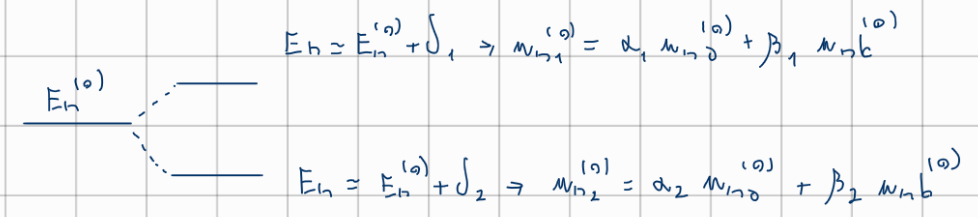
\includegraphics[width=0.7\linewidth]{immagini/2026-05-22-15-46-47.png}
    \end{figure}

\begin{quote}
    \textbf{Attenzione concettuale:} Queste nuove funzioni d'onda $u_{n_1}^{(0)}$ e $u_{n_2}^{(0)}$ che abbiamo trovato \textbf{NON SONO CORREZIONI} della funzione d'onda! % \\
    Restano pur sempre autostati dell'Hamiltoniana imperturbata $\hat{H}^{(0)}$ (cioè stati di ordine 0). % \\
    Questa procedura ci ha semplicemente fatto capire \textit{in che modo gli stati imperturbati si mescolano tra loro} per formare la base "corretta" (i "buoni autostati" di ordine zero) su cui la perturbazione può agire senza far esplodere i conti.
\end{quote}

\subsection{Degenerazione di Ordine Superiore} %

Se il livello energetico $E_n^{(0)}$ ha una degenerazione di ordine $K$ (ovvero esistono $K$ autostati linearmente indipendenti con la stessa energia), la procedura si generalizza naturalmente. %
Identifichiamo il sottospazio degenere e scriviamo l'autostato imperturbato come combinazione lineare dei $K$ stati: %
\begin{equation*}
    u_n^{(0)} = \alpha u_{n,a}^{(0)} + \beta u_{n,b}^{(0)} + \dots + k u_{n,K}^{(0)} %
\end{equation*}

\noindent
Il sistema di equazioni lineari diventa un problema agli autovalori per una matrice $K \times K$: %
\begin{equation}
    \boxed{ \begin{pmatrix} \hat{H}'_{11} & \dots & \hat{H}'_{1K} \\ \vdots & \ddots & \vdots \\ \hat{H}'_{K1} & \dots & \hat{H}'_{KK} \end{pmatrix} \begin{pmatrix} \alpha \\ \beta \\ \vdots \\ k \end{pmatrix} = E_n^{(1)} \begin{pmatrix} \alpha \\ \beta \\ \vdots \\ k \end{pmatrix} } %
\end{equation}
La risoluzione (diagonalizzazione) di questa matrice fornisce i $K$ autovalori che corrispondono alle $K$ correzioni dell'energia al primo ordine $E_n^{(1)}$. %

% --- CONTINUAZIONE: BUONI AUTOSTATI E TEOREMA DI SIMMETRIA ---

\subsection{Diagonalizzazione e "Buoni Autostati"}

Se conosciamo a priori la base che rende diagonale la perturbazione $\hat{H}'$ nel sottospazio degenere, la matrice di perturbazione assume la forma:
\begin{equation}
    \begin{pmatrix} 
        \langle u_{n1}^{(0)} | \hat{H}' | u_{n1}^{(0)} \rangle & 0 \\
        0 & \langle u_{n2}^{(0)} | \hat{H}' | u_{n2}^{(0)} \rangle 
    \end{pmatrix} 
    = \begin{pmatrix} \delta_1 & 0 \\ 0 & \delta_2 \end{pmatrix}
\end{equation}
Gli stati $|u_{n1}^{(0)}\rangle$ e $|u_{n2}^{(0)}\rangle$ che realizzano questa forma diagonale sono definiti \textbf{"buoni autostati"} (o stati di base corretti).

\begin{equation*}
\left.
\begin{aligned}
\delta_1 &= \langle n_1^{(0)} | \hat{H}' | n_1^{(0)} \rangle \\
\delta_2 &= \langle n_2^{(0)} | \hat{H}' | n_2^{(0)} \rangle
\end{aligned}
\right\} \quad \text{TEORIA NON DEGENERE}
\end{equation*}

\subsection{Il Teorema dei "Buoni Autostati"}

Possiamo identificare i "buoni autostati" senza dover diagonalizzare esplicitamente la matrice, sfruttando un teorema basato sulla commutazione degli operatori.\\

\noindent
\textbf{Teorema:}
Sia $\hat{O}$ un operatore tale che $[\hat{O}, \hat{H}^{(0)}] = 0$ e $[\hat{O}, \hat{H}'] = 0$.
Se $|u_{n1}^{(0)}\rangle$ e $|u_{n2}^{(0)}\rangle$ sono autostati di $\hat{O}$ con autovalori distinti ($\xi \neq \nu$):
\begin{equation}
    \hat{O} |u_{n1}^{(0)}\rangle = \xi |u_{n1}^{(0)}\rangle, \quad \hat{O} |u_{n2}^{(0)}\rangle = \nu |u_{n2}^{(0)}\rangle
\end{equation}
Allora l'elemento di matrice fuori diagonale della perturbazione è nullo:
\begin{equation}
    \langle u_{n1}^{(0)} | \hat{H}' | u_{n2}^{(0)} \rangle = 0
\end{equation}
Pertanto, la matrice di perturbazione è \textbf{già diagonale} nella base degli autostati di $\hat{O}$.\\

\noindent
\textbf{Dimostrazione:}
Consideriamo il commutatore $[\hat{O}, \hat{H}'] = 0$. Calcoliamo l'elemento di matrice tra i due stati:
\begin{align*}
    \langle u_{n1}^{(0)} | [\hat{O}, \hat{H}'] | u_{n2}^{(0)} \rangle &= 0 \\
    \langle u_{n1}^{(0)} | \hat{O} \hat{H}' | u_{n2}^{(0)} \rangle - \langle u_{n1}^{(0)} | \hat{H}' \hat{O} | u_{n2}^{(0)} \rangle &= 0 \\
    \xi \langle u_{n1}^{(0)} | \hat{H}' | u_{n2}^{(0)} \rangle - \nu \langle u_{n1}^{(0)} | \hat{H}' | u_{n2}^{(0)} \rangle &= 0 \\
    (\xi - \nu) \langle u_{n1}^{(0)} | \hat{H}' | u_{n2}^{(0)} \rangle &= 0
\end{align*}
Poiché per ipotesi gli autovalori sono distinti ($\xi - \nu \neq 0$), l'unica soluzione possibile è che l'elemento di matrice sia nullo.

\end{document}